\section{Implementación}

El desarrollo del sistema ha supuesto un proceso iterativo en el que se han combinado técnicas de inteligencia artificial generativa, diseño de arquitectura modular y principios de integración software. El objetivo principal ha sido construir una solución capaz de generar imágenes a partir de descripciones textuales, integrándola de forma fluida en la plataforma Java Multimedia Retrieval (JMR). Para lograrlo, se abordaron distintas fases de implementación: desde la creación de una API REST funcional y flexible en Python, hasta la extensión del cliente JMR en Java para aprovechar dicho sistema generativo. 

El detalle completo de la implementación a nivel de código no se incluye en esta memoria, ya que el objetivo es presentar una visión general de la arquitectura, las decisiones técnicas y los retos abordados durante el desarrollo. Para consultar la implementación completa, incluyendo los scripts de entrenamiento, el servidor de inferencia, la integración con JMR y la interfaz gráfica, se han habilitado tres repositorios independientes en GitHub: \texttt{TFG}, \texttt{TFG-JMR} y \texttt{TFG-UI}, todos ellos accesibles bajo solicitud al usuario \texttt{carlotiii30}.

Los enlaces y descripciones detalladas de estos repositorios pueden consultarse en el \autoref{sec:codigo-fuente}.

\subsection{Implementación de la API para la Generación de Imágenes}
Uno de los objetivos principales del proyecto fue desarrollar un sistema que permitiera la generación de imágenes a partir de descripciones textuales, accesible desde la plataforma JMR. Para ello, se implementó una API REST utilizando el framework \textit{FastAPI}, que actúa como puente entre el sistema generativo y la interfaz de usuario.

\subsubsection{Arquitectura de la API}
La API está diseñada para ser modular, escalable y fácil de integrar en otros sistemas. Se compone de los siguientes módulos:

\begin{itemize}
    \item \textbf{Módulo de generación de imágenes}: Invoca al modelo de difusión para generar imágenes a partir de texto.
    \item \textbf{Módulo de gestión de modelos}: Permite subir, eliminar o listar modelos disponibles en el sistema.
    \item \textbf{Interfaz RESTful}: Expone los endpoints que facilitan la comunicación con el sistema.
\end{itemize}

\subsubsection{Endpoints implementados}
\paragraph{Generación de imágenes}
\begin{itemize}
    \item \textbf{POST /images/generate/}
    \begin{itemize}
        \item \textbf{Descripción:} genera una imagen a partir de una descripción textual.
        \item \textbf{Entrada (JSON):}
        \begin{itemize}
            \item \texttt{model\_name} (opcional, por defecto \texttt{stable\_modified})
            \item \texttt{prompt} (requerido)
            \item \texttt{num\_inference\_steps} (opcional, por defecto 50)
            \item \texttt{guidance\_scale} (opcional, por defecto 7.5)
        \end{itemize}
        \item \textbf{Salida:} JSON con la ruta de la imagen generada.
    \end{itemize}

    \item \textbf{GET /images/download/\{image\_name\}}
    \begin{itemize}
        \item \textbf{Descripción:} descarga una imagen generada.
        \item \textbf{Entrada:} nombre del archivo.
        \item \textbf{Salida:} archivo binario de imagen.
    \end{itemize}
\end{itemize}

\paragraph{Gestión de modelos}
\begin{itemize}
    \item \textbf{POST /models/upload/}
    \begin{itemize}
        \item \textbf{Descripción:} permite subir un nuevo modelo en formato ZIP.
        \item \textbf{Entrada:} archivo ZIP.
        \item \textbf{Salida:} JSON de confirmación y ruta del modelo.
    \end{itemize}

    \item \textbf{DELETE /models/delete/\{model\_name\}}
    \begin{itemize}
        \item \textbf{Descripción:} elimina un modelo previamente subido.
        \item \textbf{Entrada:} nombre del modelo.
        \item \textbf{Salida:} mensaje de confirmación.
    \end{itemize}

    \item \textbf{GET /models/list/}
    \begin{itemize}
        \item \textbf{Descripción:} devuelve un listado de todos los modelos disponibles.
        \item \textbf{Entrada:} ninguna.
        \item \textbf{Salida:} JSON con los nombres de los modelos.
    \end{itemize}
\end{itemize}

\subsubsection{Flujo de interacción}
El usuario introduce una descripción textual en la interfaz de JMR. Esta es enviada mediante un endpoint POST a la API, que responde con una imagen generada. La API también permite gestionar modelos a través de otros endpoints, manteniendo así un sistema flexible y ampliable.

\subsubsection{Conclusión}
La API desarrollada con FastAPI proporciona una interfaz sólida y extensible para la generación de imágenes. Su diseño modular permite una integración fluida con la plataforma JMR, facilitando la evolución futura del sistema y permitiendo su adaptación a nuevos modelos o mejoras.

\subsection{Integración con la plataforma JMR (Java)}

Una parte clave del proyecto ha sido extender la plataforma Java Multimedia Retrieval (JMR) para permitir la generación de imágenes a partir de descripciones textuales. Esta funcionalidad ha sido implementada respetando la arquitectura modular existente y proporcionando una experiencia de usuario coherente con el resto del sistema.

\subsubsection{Arquitectura de integración}

El flujo completo de integración entre la interfaz y el sistema generativo se basa en la arquitectura descrita previamente en la Figura~\ref{fig:clases-java}. Según dicho esquema, la estructura se traduce en una serie de componentes interconectados que permiten gestionar el envío de prompts, la visualización de resultados y la reutilización de imágenes generadas.

A continuación se describen los principales elementos que componen esta arquitectura:

\begin{itemize}
    \item \textbf{Clase \texttt{MainWindow}}: se encarga de inicializar los componentes principales de la interfaz. Gestiona el cambio entre API local y online mediante un sistema de menús interactivo, permitiendo introducir un token cuando se selecciona la API online.
    
    \item \textbf{Clase \texttt{PromptWindow}}: ventana interna dedicada a la generación de imágenes. Incluye un cuadro de texto para el prompt, una imagen por defecto y un botón para lanzar la generación. La imagen generada se actualiza en la misma ventana, y el prompt se guarda automáticamente.

    \item \textbf{Clase \texttt{InternalWindow}}: subclase personalizada de ventana interna que permite visualizar las imágenes generadas y contiene la lógica necesaria para gestionarlas (título, visualización, reuso, etc.).

    \item \textbf{Clase \texttt{ImagePromptItem} y \texttt{ImagePromptListRenderer}}: definen la estructura visual y funcional del historial. Cada entrada del historial representa un par imagen-prompt, y puede seleccionarse para su reutilización.

    \item \textbf{Clase \texttt{ListInternalWindow}}: muestra visualmente los resultados de una consulta en la base de datos a partir de una imagen generada, en el caso de realizar una búsqueda sin visualización explícita.
\end{itemize}

\subsubsection{Flujo de generación de imagen}

Cuando el usuario accede a la opción \texttt{Generar Imagen}, se abre una instancia de \texttt{PromptWindow}. Esta ventana contiene:

\begin{itemize}
    \item Un cuadro de texto para introducir la descripción (prompt).
    \item Una imagen de marcador por defecto.
    \item Un botón que al pulsarse envía una petición HTTP a la API REST configurada (local u online) usando el prompt indicado.
\end{itemize}

La respuesta es una imagen en binario que se muestra en la misma ventana y se almacena localmente. Además, se añade una nueva entrada al historial mediante una instancia de \texttt{ImagePromptItem}, que queda registrada para consultas posteriores desde un menú desplegable.

\subsubsection{Selección y gestión de la API}

Desde el menú superior de la clase \texttt{MainWindow}, el usuario puede seleccionar si desea usar una API local o remota:

\begin{itemize}
    \item Al seleccionar \texttt{Online API}, se abre un cuadro de diálogo solicitando un token. Si se proporciona correctamente, se guarda para las siguientes peticiones.
    \item Si se cancela o el token es inválido, el sistema vuelve automáticamente a \texttt{Local API}.
\end{itemize}

Este mecanismo asegura que la opción activa siempre sea válida, y se mantiene durante toda la sesión.

\subsubsection{Consulta sin visualización}

En el caso de realizar una consulta directa (sin mostrar la imagen), el prompt se toma del cuadro de texto principal y se lanza una generación en segundo plano. La imagen generada se usa como entrada para una búsqueda visual mediante el motor de recuperación de JMR. Los resultados se muestran en una instancia de \texttt{ListInternalWindow}, sin mostrar la imagen generada al usuario.

\subsubsection{Historial reutilizable}

El historial se gestiona mediante una lista desplegable que utiliza un renderizador personalizado para mostrar cada entrada de forma clara y compacta. El usuario puede:

\begin{itemize}
    \item Visualizar entradas previas seleccionándolas desde el historial.
    \item Reabrir la imagen correspondiente en una nueva \texttt{InternalWindow}.
    \item Consultar la descripción asociada al pasar el cursor por encima.
\end{itemize}

Este historial se actualiza dinámicamente cada vez que se genera una nueva imagen.

\subsubsection{Gestión de errores}

Se han implementado cuadros de diálogo para mostrar mensajes claros ante situaciones como:

\begin{itemize}
    \item Prompt vacío o inválido.
    \item Fallo de conexión con la API.
    \item Token incorrecto.
    \item Imagen generada no disponible en disco.
    \item Estructura inválida del modelo cargado.
\end{itemize}

Estas validaciones mejoran la robustez y evitan que el sistema se bloquee ante entradas inesperadas.

\subsubsection{Comunicación con el sistema generativo: descriptores de imagen}

La integración entre la interfaz de usuario y la API REST del sistema generativo se estructura en torno a una jerarquía de clases que encapsulan el proceso de generación de imágenes a partir de texto. Esta arquitectura, representada en la \autoref{fig:clases-python}, permite abstraer los detalles técnicos de la comunicación con el backend, garantizando una interfaz uniforme y extensible.

A continuación se describen las clases principales:

\begin{itemize}
    \item \textbf{\texttt{AbstractPromptImageDescriptor}}: clase base que define el comportamiento común a todos los descriptores basados en texto. Contiene los campos necesarios para almacenar el prompt, el nombre del modelo empleado y la imagen generada (de tipo \texttt{BufferedImage}). Define además el método abstracto \texttt{generate()}, que debe ser implementado por las subclases para llevar a cabo el proceso de generación correspondiente.

    \item \textbf{\texttt{PromptGeneratedImageDescriptor}}: implementación para generación remota. El método \texttt{generate()} realiza una petición HTTP POST al endpoint \texttt{/images/generate/}, enviando los datos del prompt y del modelo. Como respuesta, recibe una ruta relativa de la imagen generada, que posteriormente se descarga mediante un GET a \texttt{/images/download/\{filename\}}.

    \item \textbf{\texttt{PromptGeneratedImageDescriptorLocal}}: implementación para generación local, en entornos donde la API está desplegada en localhost. Aunque reutiliza la lógica de generación remota, modifica la URL base y simplifica el flujo de validación al no depender de red.
\end{itemize}

La clase \texttt{MainWindow} se encarga de instanciar el descriptor adecuado en función del modo seleccionado por el usuario (API local u online), sin que el resto de la aplicación tenga que preocuparse por los detalles de la comunicación. Esta separación de responsabilidades permite que otros componentes, como los encargados de mostrar o guardar imágenes, interactúen con los descriptores de forma homogénea a través del método \texttt{getGeneratedImage()}, que garantiza que la imagen ha sido generada y devuelve un objeto \texttt{BufferedImage} listo para ser usado.

Gracias a esta arquitectura, el sistema es fácilmente extensible. Es posible incorporar nuevos tipos de descriptores, ya sea para otros modelos generativos o servicios externos, sin necesidad de modificar la lógica central de la aplicación. Además, al encapsular dentro de cada descriptor la gestión de errores y validaciones, se facilita el mantenimiento del código y se mejora la robustez del sistema.


\subsection{Consideraciones de seguridad y rendimiento}

Durante el desarrollo del sistema de generación de imágenes, se han contemplado múltiples aspectos relacionados con la seguridad del servicio, la gestión del entorno de ejecución, la optimización del rendimiento y la preparación para entornos de producción. Estas consideraciones resultan fundamentales para garantizar la integridad de los datos, la reproducibilidad de los experimentos y la escalabilidad futura del sistema en contextos reales.

\subsubsection{Gestión del entorno con Poetry}

Para asegurar un entorno de ejecución reproducible, coherente y fácilmente desplegable, se ha utilizado \textbf{Poetry} como gestor de dependencias y empaquetado. Esta herramienta ha permitido:

\begin{itemize}
    \item Especificar con precisión las versiones de todas las librerías utilizadas, como \texttt{diffusers}, \texttt{transformers}, \texttt{torch}, \texttt{Pillow}, entre otras, evitando incompatibilidades entre ellas.
    \item Garantizar la replicabilidad del entorno en distintas máquinas mediante los archivos \texttt{pyproject.toml} y \texttt{poetry.lock}, facilitando el trabajo colaborativo o la migración a servidores externos.
    \item Aislar completamente el entorno de desarrollo de otras instalaciones globales de Python, reduciendo el riesgo de conflictos entre proyectos.
    \item Preparar el proyecto para su distribución como paquete Python, en caso de que se quisiera liberar o integrar como dependencia en otros sistemas.
\end{itemize}

\subsubsection{Contenerización y portabilidad con Docker}

Para facilitar el despliegue del sistema en distintos entornos (local, servidor o nube), se ha incorporado \textbf{Docker} como herramienta de contenerización. Esto ha permitido encapsular todo el entorno de ejecución en una imagen portátil y reproducible, con las siguientes ventajas:

\begin{itemize}
    \item Elimina dependencias externas del sistema operativo anfitrión, asegurando que todas las versiones de librerías y herramientas se mantengan consistentes.
    \item Facilita el despliegue del sistema en servidores remotos, entornos cloud o plataformas de orquestación como Kubernetes.
    \item Permite realizar pruebas locales sin afectar al entorno del desarrollador.
    \item Mejora la seguridad al encapsular los procesos y evitar accesos arbitrarios al sistema anfitrión.
\end{itemize}

El archivo \texttt{Dockerfile} define el entorno con precisión, incluyendo la instalación de \texttt{poetry}, las dependencias del proyecto y la ejecución del servidor con \texttt{uvicorn}. Para facilitar la ejecución, se han definido scripts automatizados que permiten iniciar el contenedor con un solo comando.

Esta estrategia prepara el sistema para un despliegue más robusto y escalable en futuras fases del proyecto.

\subsubsection{Seguridad en la API REST}

Dado que el sistema de generación se expone a través de una interfaz web (API REST), es fundamental considerar posibles vectores de ataque relacionados con el envío de solicitudes maliciosas, el uso no autorizado o la exposición de recursos sensibles. Aunque esta versión del sistema no incluye mecanismos avanzados de autenticación o autorización, se han implementado algunas medidas preliminares de validación estructural y se identifican los siguientes aspectos clave para futuras iteraciones:

\begin{itemize}
    \item \textbf{Validación de entradas:} actualmente, FastAPI permite tipado estático de parámetros, pero no se han definido aún restricciones estrictas sobre la longitud o estructura de los textos recibidos. Esto puede derivar en uso abusivo o errores inesperados ante entradas malformadas. Se recomienda implementar validaciones adicionales a nivel de contenido y lógica.
    
    \item \textbf{Validación de estructura de modelos:} se ha incorporado un sistema de validación estructural para los modelos subidos por el usuario. Esta validación, implementada mediante la función, comprueba que la carpeta del modelo contenga todos los subdirectorios y archivos esperados —como \texttt{config.json}, \texttt{model.safetensors}, o \texttt{tokenizer\_config.json}—. Si falta alguno de estos elementos, se lanza una excepción \texttt{HTTPException} con un código de error 400, evitando así el uso de modelos incompletos o manipulados que puedan comprometer el funcionamiento del sistema.

    \item \textbf{Control del acceso a archivos:} actualmente no se ha desarrollado un sistema de permisos que restrinja el acceso directo a imágenes generadas o modelos almacenados. El sistema confía en una organización interna de rutas, lo cual no es suficiente para prevenir accesos arbitrarios si la API se expusiera públicamente. Se recomienda proteger los endpoints y establecer rutas temporales con tokens de acceso.

    \item \textbf{Límites de uso:} el servicio no impone cuotas por usuario, IP ni número de peticiones. En un entorno expuesto, esto puede derivar en ataques de denegación de servicio (DoS) o consumo excesivo de recursos. Se recomienda implementar mecanismos como rate limiting, autenticación básica o tokens temporales.

    \item \textbf{Manejo de errores:} aunque FastAPI ofrece gestión automática de errores comunes, no se ha personalizado la respuesta ante excepciones críticas. Actualmente, algunos errores podrían devolver trazas del servidor, lo que podría exponer rutas internas o detalles sensibles del sistema. Se sugiere capturar explícitamente excepciones clave y devolver mensajes controlados y neutros.
\end{itemize}

En resumen, aunque el sistema aún no está preparado para un entorno productivo expuesto, ya se han incorporado medidas preventivas como la validación estructural de modelos, que garantiza la integridad mínima antes de permitir su ejecución. Estas medidas constituyen una base sobre la que construir mecanismos más robustos de autenticación, protección de recursos y resiliencia frente a ataques externos.

Todas estas cuestiones han sido tenidas en cuenta de cara a un posible despliegue en producción. Se recomienda como trabajo futuro incorporar autenticación de usuarios, límites de uso, logs de auditoría y un tratamiento más robusto de la validación de parámetros para proteger el sistema frente a usos indebidos.


\subsubsection{Optimización del rendimiento}

Para maximizar la eficiencia del sistema, especialmente en entornos con recursos limitados, se han llevado a cabo diversas estrategias:

\begin{itemize}
    \item \textbf{Carga única del modelo}: el modelo generativo se inicializa una única vez al arrancar el servidor, evitando recargas innecesarias en cada solicitud.
    \item \textbf{Uso eficiente del espacio en disco}: las imágenes generadas se almacenan temporalmente en disco con nombres únicos, y se reutilizan si ya existen para un mismo prompt y configuración.
    \item \textbf{Configuración adaptable}: aunque se ha utilizado \texttt{float32} durante el desarrollo, el sistema está preparado para funcionar con \texttt{float16} o \texttt{bfloat16} en entornos con soporte, permitiendo reducir a la mitad el uso de memoria sin pérdida significativa de calidad.
    \item \textbf{Pipeline modular}: la arquitectura permite cambiar fácilmente el modelo base, el VAE o el codificador de texto, permitiendo futuras mejoras sin afectar al resto del sistema.
\end{itemize}

\subsubsection{Preparación para producción y despliegue escalable}

Aunque el presente sistema ha sido desarrollado en un entorno controlado, se han identificado y documentado las acciones necesarias para su migración a entornos reales de producción. Entre las medidas consideradas:

\begin{itemize}
    \item \textbf{Autenticación}: implementación de tokens JWT para identificar usuarios y restringir el acceso a usuarios registrados.
    \item \textbf{Rate limiting}: limitación de solicitudes por IP o por usuario en función de cuotas diarias o mensuales.
    \item \textbf{Contenerización}: uso de Docker para encapsular el entorno, garantizando portabilidad y facilitando el despliegue en VPS, Kubernetes o servicios cloud.
    \item \textbf{Proxy inverso con Caddy o NGINX}: para mejorar la seguridad en las conexiones HTTP y permitir balanceo de carga entre instancias.
    \item \textbf{Logging y monitorización}: integración de herramientas de seguimiento de logs y métricas del sistema para supervisar el uso real del servicio.
\end{itemize}

\subsubsection{Reflexión final}
Estas medidas y estrategias no solo han permitido desarrollar un sistema funcional en el presente, sino que establecen las bases para una posible evolución futura hacia un servicio robusto y escalable. La combinación de buenas prácticas en gestión de entornos, principios básicos de seguridad y una arquitectura eficiente posiciona este proyecto como un prototipo avanzado, listo para crecer hacia escenarios reales de uso y despliegue institucional o comercial.


\subsection{Pruebas y validación}

Para validar el correcto funcionamiento del sistema desarrollado, se han realizado pruebas tanto sobre la API REST de generación como sobre la integración completa dentro de la plataforma Java JMR. Estas pruebas tenían como objetivo verificar la funcionalidad de los endpoints, la integridad del flujo de generación, la correcta gestión del historial y la interacción con la base de datos visual.

\subsubsection{Pruebas sobre la API REST}

La API desarrollada con \texttt{FastAPI} cuenta con una interfaz interactiva (Swagger UI), accesible en \texttt{/docs}, desde la cual es posible probar directamente todos los endpoints definidos. Se realizaron pruebas manuales de los principales puntos del sistema:

\begin{itemize}
    \item \textbf{GET /models/list/}: verifica que la API devuelve correctamente los modelos disponibles. En la prueba, se recibió el modelo por defecto \texttt{"stable"}.

    \item \textbf{POST /images/generate/}: permite generar una imagen a partir de un prompt textual. En la prueba realizada se utilizó el prompt \textit{"a sunset on the beach"} con parámetros por defecto. La respuesta fue satisfactoria, devolviendo el nombre del archivo generado.

    \item \textbf{GET /images/download/\{image\_name\}}: descarga la imagen generada, lo que permitió comprobar la existencia y legibilidad del archivo.

    \item \textbf{Manejo de errores}: se realizaron pruebas con modelos inexistentes, prompts vacíos o estructuras incorrectas. La API devolvió códigos HTTP coherentes (400 o 422) y mensajes de error controlados, como se especifica en la validación estructural.
\end{itemize}

\begin{figure}[H]
    \centering
    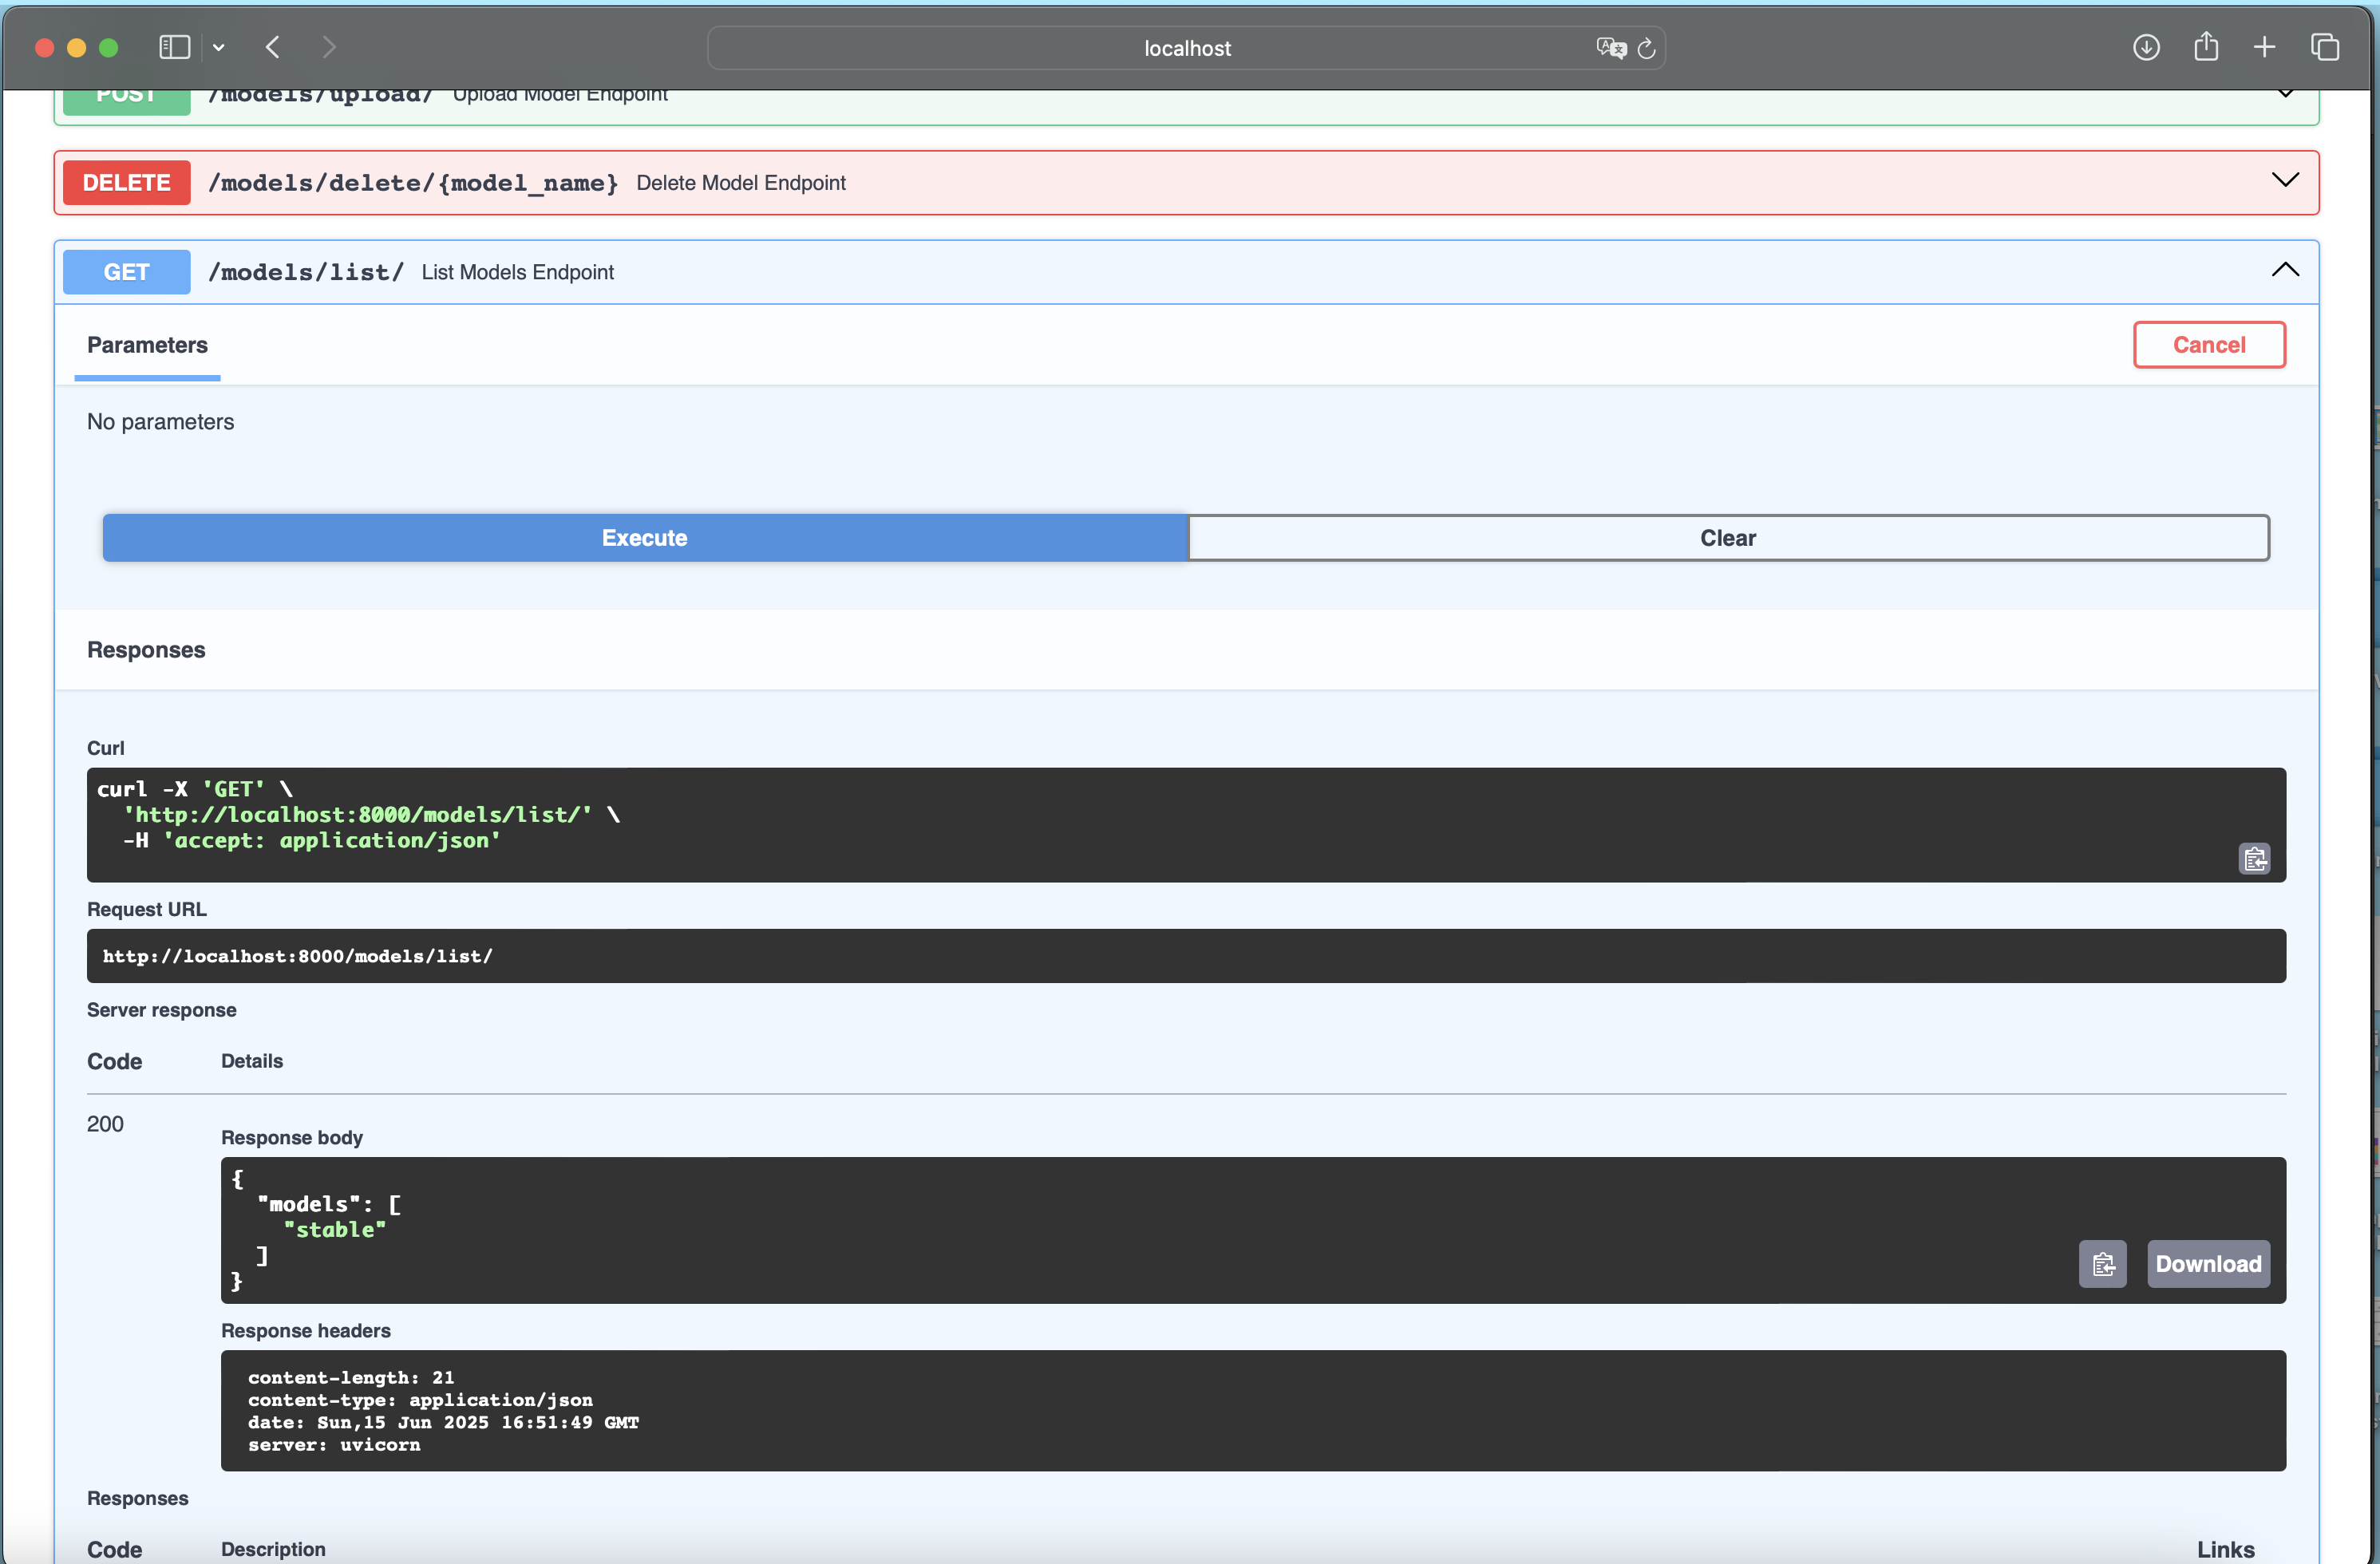
\includegraphics[width=0.6\textwidth]{api/list_models.png}
    \caption{Prueba del endpoint \texttt{GET /models/list/} desde Swagger}
\end{figure}

\begin{figure}[H]
    \centering
    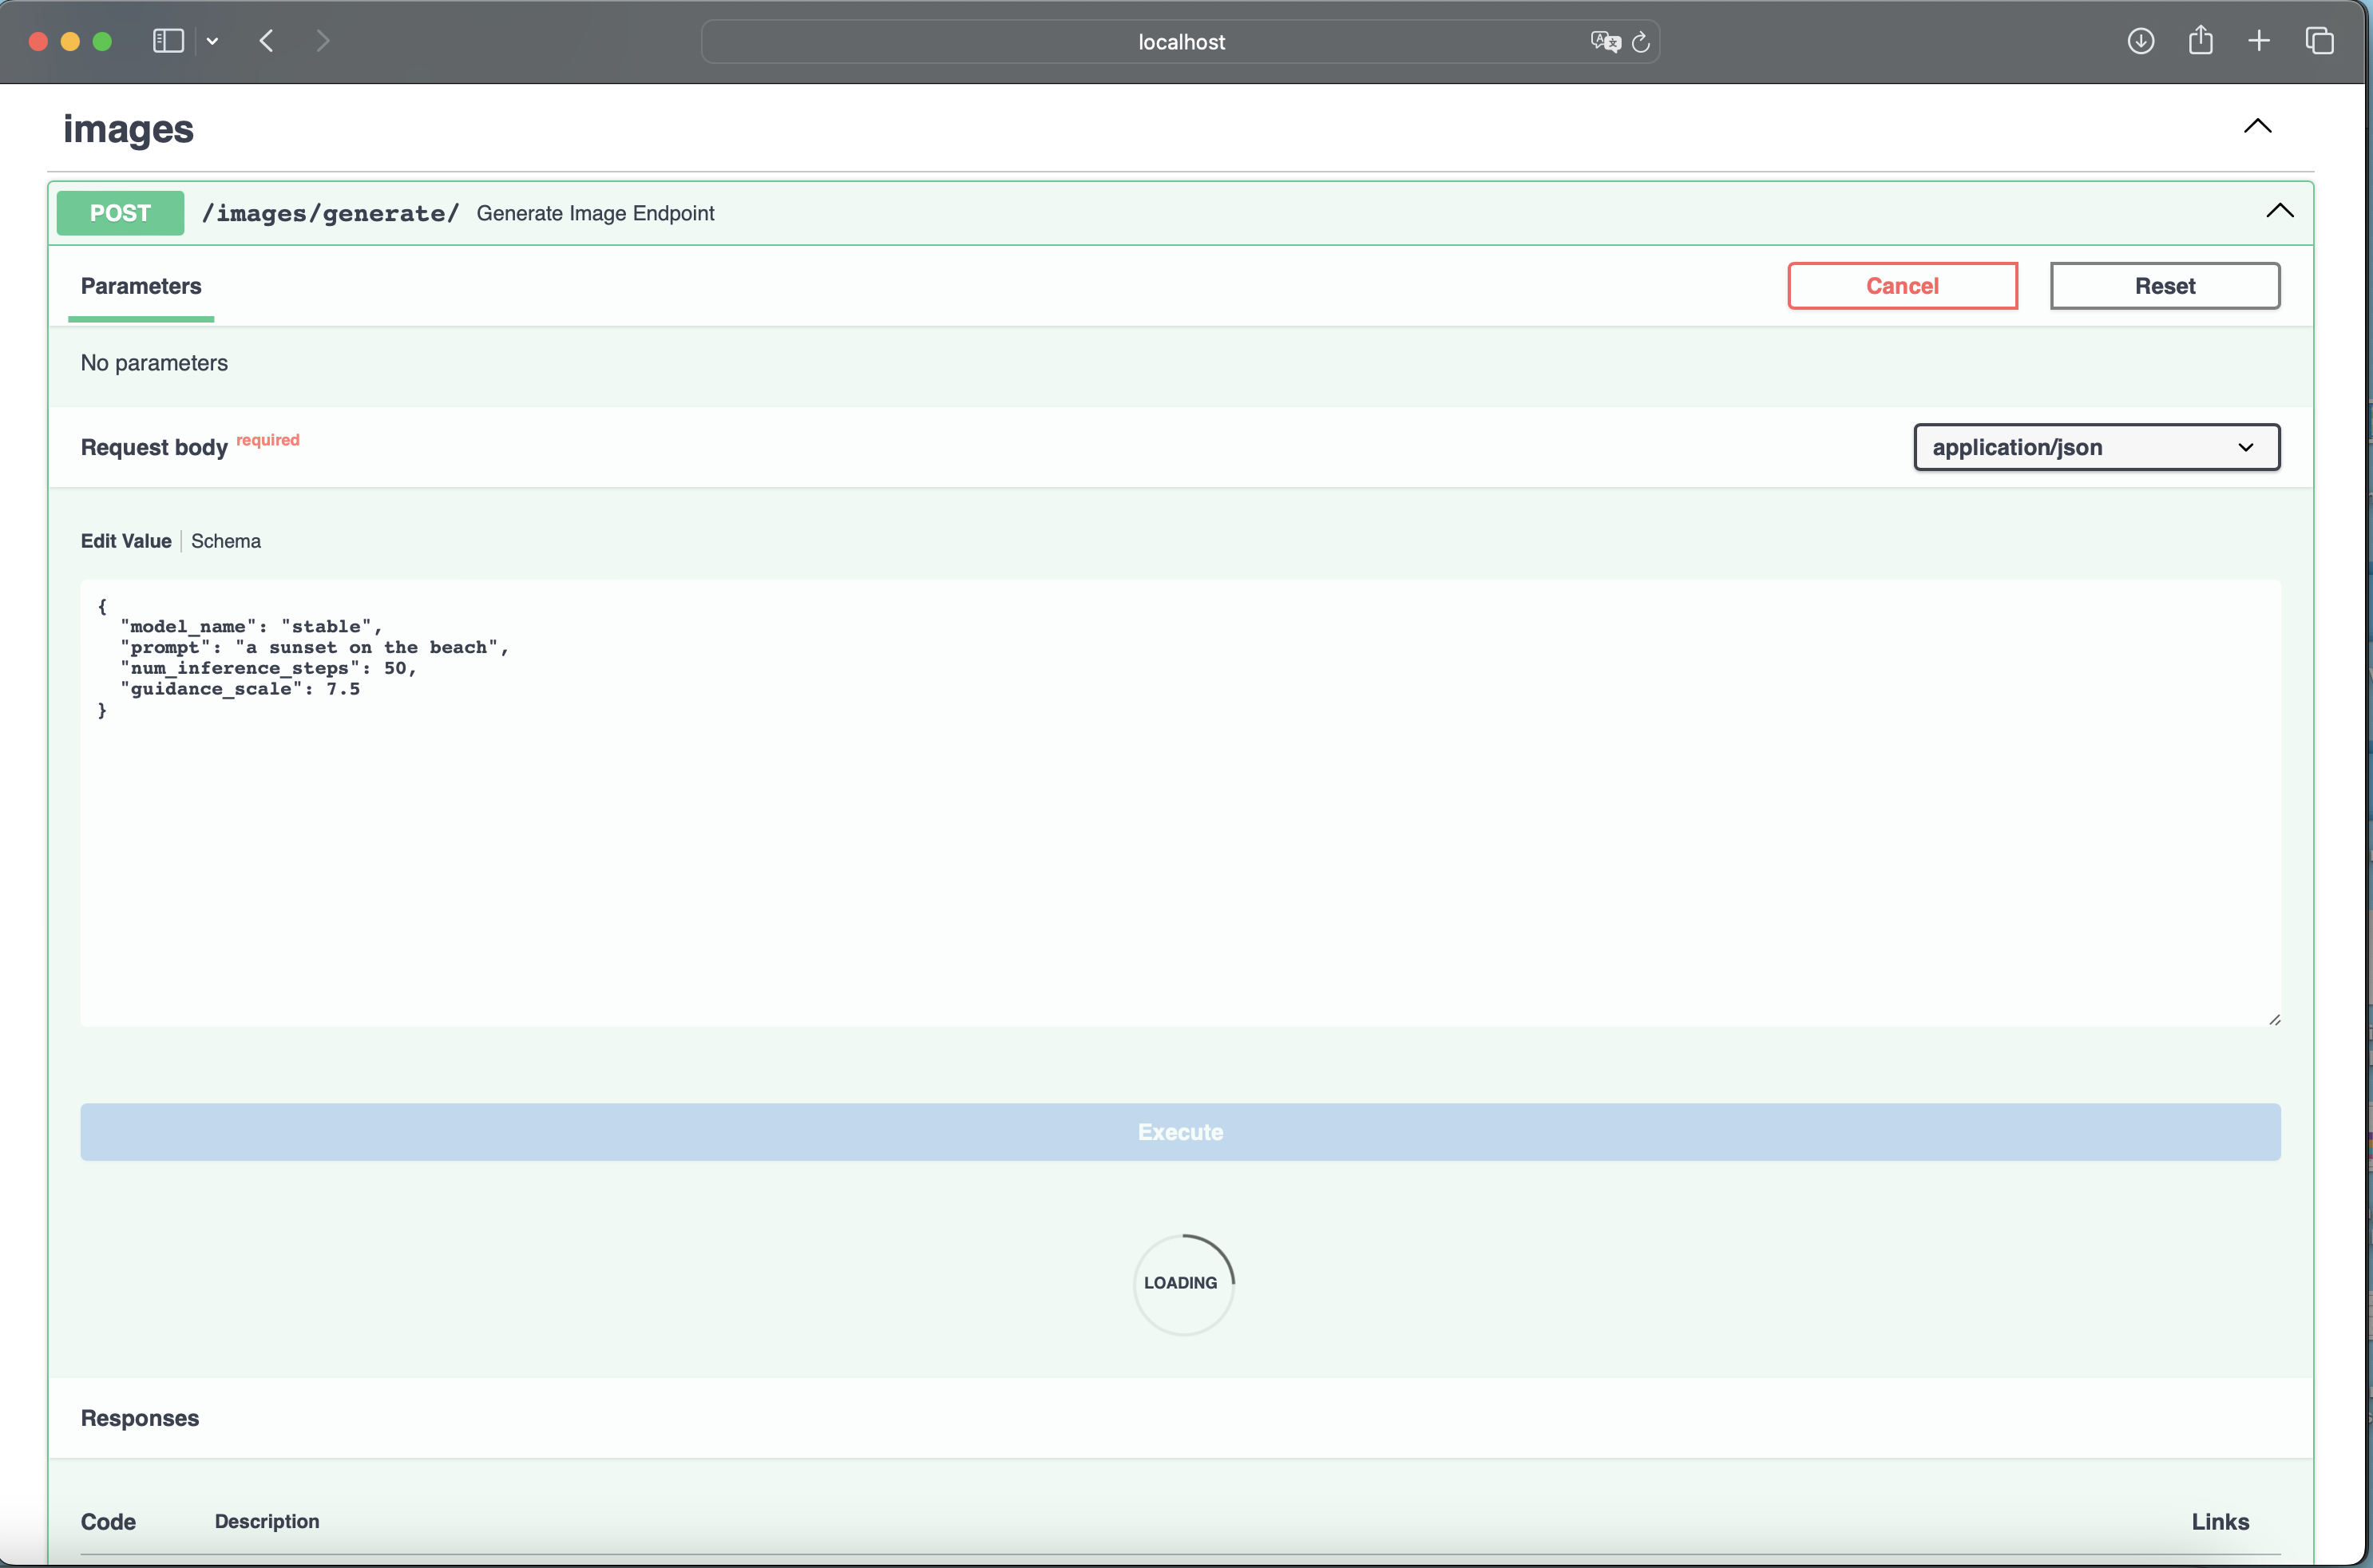
\includegraphics[width=0.6\textwidth]{api/generate_image.png}
    \caption{Prueba del endpoint \texttt{POST /images/generate/} con prompt textual}
\end{figure}

Además de estas pruebas manuales, se desarrollaron tests automáticos utilizando \texttt{pytest} para las funciones internas del servidor, incluyendo validaciones sobre el manejo de prompts, la existencia del modelo solicitado y la correcta generación y localización de las imágenes. Estos tests permitieron asegurar la estabilidad del sistema ante cambios futuros y facilitar su mantenimiento.


\subsubsection{Pruebas en la aplicación JMR}

La validación funcional dentro de la interfaz gráfica de JMR se llevó a cabo comprobando las siguientes funcionalidades:

\begin{itemize}
    \item \textbf{Selección de API local/online}: se comprobó que el sistema gestionaba correctamente el cambio entre API, solicitando el token cuando era necesario y manteniendo el estado activo durante la sesión.

    \item \textbf{Generación desde interfaz}: se probó la creación de una imagen a partir de un prompt, observando la aparición automática en la ventana interna junto con la actualización del historial.

    \item \textbf{Consulta sin visualización}: se utilizó el cuadro de texto superior para lanzar una búsqueda desde descripción sin visualizar la imagen. El sistema generó correctamente la imagen en segundo plano y devolvió los resultados similares en la base de datos.

    \item \textbf{Historial de imágenes}: se validó que las entradas quedaban correctamente almacenadas, eran accesibles desde el desplegable, y al seleccionarlas se abría la ventana correspondiente.

    \item \textbf{Reutilización de imágenes generadas}: se reutilizaron imágenes del historial para lanzar nuevas consultas, sin volver a generar los archivos en disco.

    \item \textbf{Errores controlados}: se forzaron errores como prompts vacíos, imágenes eliminadas o modelos mal estructurados, observando que el sistema respondía con mensajes claros sin bloquear la aplicación.
\end{itemize}

\begin{figure}[H]
    \centering
    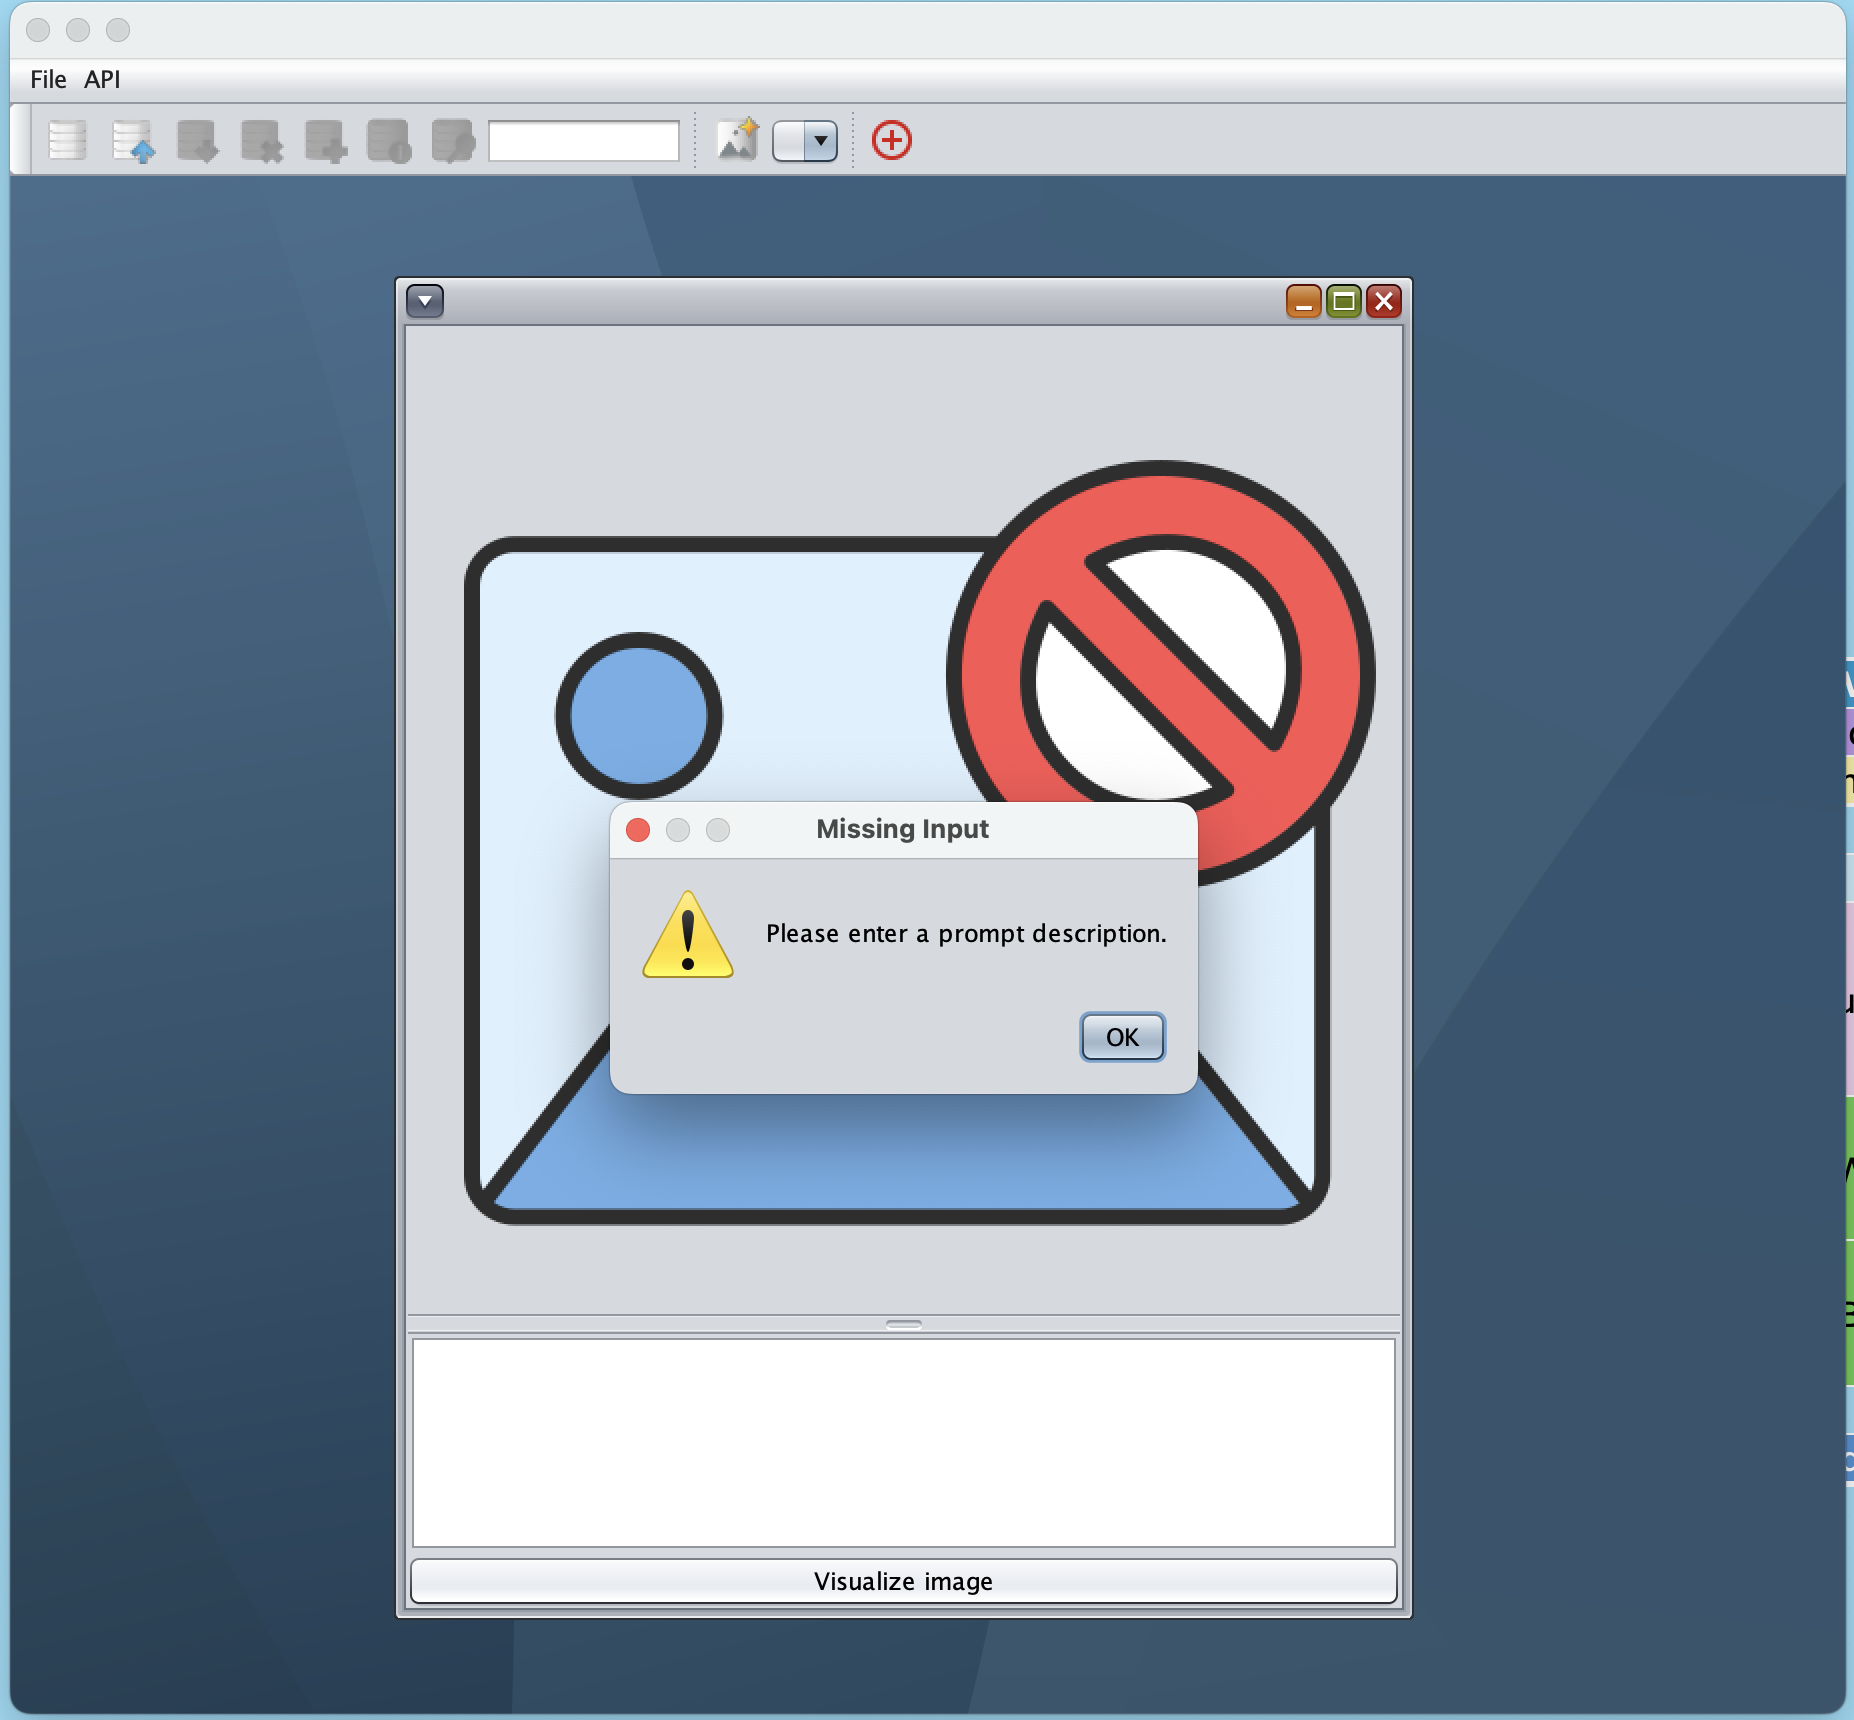
\includegraphics[width=0.45\textwidth]{api/prompt_vacio.png}
    \caption{Mensaje de error al intentar generar un prompt vacío}
\end{figure}

\subsubsection{Validación de consistencia e integridad}

Para confirmar que el sistema funcionaba de forma coherente y sin redundancias, se realizaron pruebas cruzadas:

\begin{itemize}
    \item Se compararon imágenes generadas con prompts similares para validar la coherencia del modelo.
    \item Se comprobó que no se duplicaban archivos si se reutilizaba el mismo prompt.
    \item Se examinó el rendimiento en generación en entorno local y se registró el tiempo medio de respuesta.
\end{itemize}

\subsubsection{Conclusión}

Las pruebas realizadas han demostrado que el sistema es funcional, coherente y robusto en entornos controlados. La API responde adecuadamente ante entradas válidas y malformadas, mientras que la integración con JMR mantiene una experiencia fluida para el usuario final. Aunque aún pueden incorporarse mecanismos adicionales de seguridad y autenticación, el sistema se encuentra en un estado válido para su uso en escenarios de validación funcional y pruebas de concepto.
